\section{Задание 1}

Введите свою фамилию, пол и возраст

\begin{center} 
  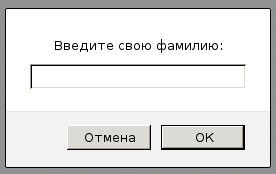
\includegraphics[width=9cm]{img/01.png}
  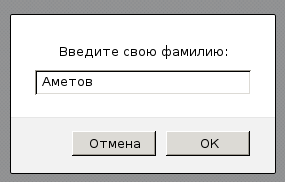
\includegraphics[width=9cm]{img/02.png}
  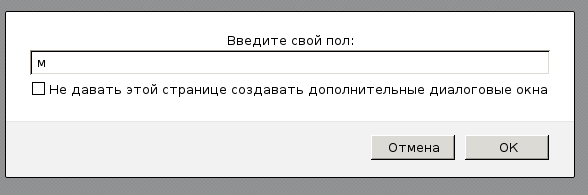
\includegraphics[width=9cm]{img/03.png}
  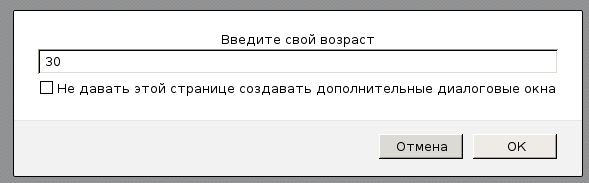
\includegraphics[width=9cm]{img/04.png}
\end{center}

Запросите подтверждение

\begin{center} 
  
\includegraphics[width=9cm]{img/05.png}
\end{center}

Если всё верно, то вывести приветствие, если нет, вывести сообщение об ошибке:

\begin{center} 
  
\includegraphics[width=9cm]{img/06.png}
  
\includegraphics[width=9cm]{img/07.png}
\end{center}

Исходный код \verb|exercise_01_v2.html|:
\begin{verbatim}
<body>
  <head>
    <meta charset = "utf-8">
  </head>
  <script>
    surname = prompt ("Введите свою фамилию:")
    sex = prompt ("Введите свой пол:", "м")
    age = parseInt (prompt ("Введите свой возраст", "0"))
    result = confirm ("ФИО: " + surname + "\n" + "Пол: " + sex +
    "\n" + "Возраст: " + age + "\n" + "Всё верно?");
    if (result) alert ("Молодец, " + surname + "!")
    else alert ("Ошибка в данных");
  </script>
</body>
\end{verbatim}
